%!TEX program = lualatex
\PassOptionsToPackage{usenames, dvipsnames}{color}
\documentclass{aleph-revista}
\usepackage{fontspec}
\setmainfont{Times New Roman}
\usepackage{unicode-math}
\setmathfont{TeX Gyre Termes Math}
\usepackage{tikz}
\usepackage{graphicx}
\usepackage{aleph-comandos} 
\usepackage{multicol}    
\usepackage[usenames]{color}
\usepackage{parskip}
\usepackage{hyperref}
\usepackage[spanish]{babel}
\usepackage{amsmath, amssymb, amsthm, mathrsfs}
\usepackage{enumitem}
\newtheorem{proposition}{Proposición}
\newtheorem{lemma}{Lema}

\hypersetup{
    colorlinks=true,
    linkcolor=blue,
    filecolor=blue,      
    urlcolor=cyan,
    pdftitle={Sharelatex Example},
    pdfpagemode=FullScreen,
    }
\addbibresource{bibliografia.bib}

% Fourier
% hat y widecheck
\DeclareFontFamily{U}{mathx}{}
\DeclareFontShape{U}{mathx}{m}{n}{<-> mathx10}{}
\DeclareSymbolFont{mathx}{U}{mathx}{m}{n}
\providecommand{\check}{\widecheck}
\renewcommand{\hat}{\widehat}
\renewcommand{\tilde}{\widetilde}
\providecommand{\norm}[1]{\left\|#1\right\|}


\newcommand{\ident}{\hspace{0.5cm}}
\renewcommand\qedsymbol{$\blacksquare$}
\fechapubli{2025}
\periodouno{Julio}

\titulo{Estimación tipo conmutador para transformadas de Hilbert y derivadas fraccionarias.}

\tituloingles{Hilbert transform type estimation and fractional derivatives.}

\autor{Andrés David Cadena Simons}
\institucion{Universidad Nacional de Colombia, Facultad de ciencias, Sede Bogotá}
\correo{acadenas@unal.edu.co}

\fecha{\today}
\resumen{
En este trabajo se estudia una estimación de conmutador para el operador $H_x D_x^\alpha$, compuesto por la transformada de Hilbert y una derivada fraccionaria. Específicamente, se demuestra que
\begin{align*}
  \| [H_x D_x^\alpha, g] D_x^\beta f \|_{L^p} \lesssim \| \partial_x g \|_{L^\infty} \cdot \|f\|_{L^p},
\end{align*}
donde $\alpha + \beta = 1$ y $1 < p < \infty$. La demostración se desarrolla con todo detalle, descomponiendo el conmutador según los regímenes de interacción de frecuencias y utilizando herramientas del análisis armónico moderno: operadores de Littlewood–Paley, el operador maximal, el teorema de Fefferman–Stein y técnicas de estimación punto a punto. Este resultado es relevante en el contexto del análisis de ecuaciones en derivadas parciales no lineales y se relaciona con la teoría de operadores pseudo-diferenciales y de conmutadores tipo Coifman–Meyer.
}
\palabrasc{transformada de Hilbert, derivadas fraccionarias, operadores singulares, análisis armónico, conmutadores, ecuaciones dispersivas, Littlewood–Paley, estimaciones en $L^p$.}
\begin{document}
\membrete
%%%%%%%%%%%%%%%%%%%%%%%%%%%%%%%%%%%%%%%%%%%%%%%%%%%
\section{Introducción}
El objetivo de este trabajo es demostrar en detalle la siguiente estimación tipo conmutador:
\begin{proposition}[Estimación tipo conmutador no local]
Sea $1 < p < \infty$, $0 < \alpha, \beta \leq 1$, tal que $\alpha + \beta = 1$. Entonces
\begin{align*}
  \norm{D_x^{\alpha} [H_x, g] D_x^{\beta} f}_{L^p(\mathbb{R})} \lesssim_{p,\alpha,\beta} \norm{\partial_x g}_{L^\infty(\mathbb{R})}\norm{f}_{L^p(\mathbb{R})}, 
\end{align*}
para toda función $g$ suave con derivada acotada y toda $f \in \mathcal{S}(\mathbb{R})$.
\end{proposition}
%%%%%%%%%%%%%%%%%%%%%%%%%%%%%%%%%%%%%%%%%%%%%%%%%%%
\section{Preliminares}
Recordamos que la transformada de Hilbert $H_x$ está definida en la transformada de Fourier como
\begin{align*}
  \hat{H_x f}(\xi) = -isgn(\xi) \hat{f}(\xi). 
\end{align*}
Además, las derivadas fraccionarias están dadas por el operador
\begin{align*}
  \hat{D_x^s f}(\xi) = |\xi|^s \hat{f}(\xi), \qquad s \in \mathbb{R}. 
\end{align*}
También usaremos las proyecciones de Littlewood–Paley $P^x_N$ definidas por
\begin{align*}
  \hat{P^x_N f}(\xi) = \psi_N(\xi) \hat{f}(\xi), 
\end{align*}
donde $\psi_N(\xi)$ es un multiplicador suave con soporte en frecuencias de orden $|\xi| \sim N$, con $N$ número diádico.\\
Utilizaremos además las siguientes herramientas fundamentales
\begin{lemma}[Fefferman–Stein]
  Sea $f = (f_j)_{j=1}^{\infty}$ una secuencia de funciones localmente integrables en $\mathbb{R}$. Si $1 < p < \infty$, entonces
  \begin{align*}
    \norm{(Mf_j)_{l^2}}_{L^p} \leq C_p \norm{(f_j)_{l^2}}_{L^p}, 
  \end{align*}
  donde $M$ denota la función maximal de Hardy–Littlewood.
\end{lemma}
\begin{lemma}[Estimación tipo Calderón]
  Para $l + m \geq 1$, se tiene
  \begin{align*}
    \norm{\partial_x^l [H_x, g] \partial_x^m f}_{L^p} \lesssim \norm{\partial_x^{l + m} g}_{L^\infty} \norm{f}_{L^p}. 
  \end{align*}
\end{lemma}
%%%%%%%%%%%%%%%%%%%%%%%%%%%%%%%%%%%%%%%%%%%%%%%%%%
\section{Demostración de la Proposición}
Comenzamos suponiendo el caso no trivial donde $0 < \alpha, \beta < 1$ y $\alpha + \beta = 1$. El caso $\beta = 1$, $\alpha = 0$ se sigue directamente de la estimación clásica de Calderón.\\
Queremos estimar
\begin{align*}
  D_x^\alpha [H_x, g] D_x^\beta f. 
\end{align*}

\subsection*{Expresión integral del conmutador en Fourier}
  Note que por la definición de conmutador se tiene que
  \begin{align*}
    [H_x, g] D_x^\beta f = H_x(g D_x^\beta f) - g H_x D_x^\beta f. 
  \end{align*}
  Aplicamos la derivada fraccionaria
  \begin{align*}
    D_x^\alpha [H_x, g] D_x^\beta f = D_x^\alpha H_x(g D_x^\beta f) - D_x^\alpha (g H_x D_x^\beta f). 
  \end{align*}
  Usando su expresión como multiplicador se tiene que
  \begin{align*}
    \hat{\left(D_{x}^{\alpha}H_{x}(gD_{x}^{\beta}f)\right)}(\xi)&=(2\pi i)^{|\alpha|}|\xi|^{\alpha}(-i sgn(\xi))\hat{gD_{x}^{\beta}f}(\xi),\\
    &=(2\pi i)^{|\alpha|}|\xi|^{\alpha}(-i sgn(\xi))\left(\hat{g}*\hat{D_{x}^{\beta}f}\right)(\xi),\\
    &=(2\pi i)^{|\alpha|}|\xi|^{\alpha}(-i sgn(\xi))\left(\hat{g}*(2\pi i)^{|\beta|}|\xi|^{\beta}\hat{f}\right)(\xi),\\
    &=(2\pi i)^{|\alpha|+|\beta|}|\xi|^{\alpha}(-i sgn(\xi))\left(\hat{g}*|\xi|^{\beta}\hat{f}\right)(\xi),\\
    &=(2\pi i)^{|\alpha|+|\beta|}|\xi|^{\alpha}(-i sgn(\xi))\int_{-\infty}^{\infty}\hat{g}(\eta)|\xi-\eta|^{\beta}\hat{f}(\xi-\eta)\, d\eta,\\
    &=(2\pi i)^{|\alpha|+|\beta|}(-i)\int_{-\infty}^{\infty}sgn(\xi)|\xi|^{\alpha}|\xi-\eta|^{\beta}\hat{g}(\eta)\hat{f}(\xi-\eta)\, d\eta.
  \end{align*}
  De manera similar se puede llegar a que
  \begin{align*}
    \hat{\left( D_{x}^{\alpha}gH_{x}D_{x}^{\beta}f \right)}(\xi)&=(2\pi i)^{|\alpha|+|\beta|}(-i)\int_{-\infty}^{\infty}sgn(\xi-\eta)|\xi|^{\alpha}|\xi-\eta|^{\beta}\hat{g}(\eta)\hat{f}(\xi-\eta)\, d\eta.
  \end{align*}
  Siendo así, juntando ambas expresiones y realizando los cambios de variables $\eta=\xi_{1}$ y $\xi_{2}=\xi-\eta$, es decir $\xi_{1}+\xi_{2}=\xi$ podemos verificar que
  \begin{align*}
    \hat{\left( D_{x}^{\alpha}\left[ H_{x},g \right]D_{x}^{\beta}f \right)}(\xi_{1}+\xi_{2})&=(2\pi i)^{|\alpha|+|\beta|}(-i)\int_{-\infty}^{\infty}(sgn(\xi_{1}+\xi_{2})-sgn(\xi_{2}))|\xi_{1}+\xi_{2}|^{\alpha}|\xi_{2}|^{\beta}\hat{g}(\xi_{1})\hat{f}(\xi_{2})\, d\xi_{1}.
  \end{align*}
  Lo que nos permite afirmar que
  \begin{align*}
    \hspace{-1.5cm}D_{x}^{\alpha}\left[ H_{x},g \right]D_{x}^{\beta}f(x)&=(2\pi i)^{|\alpha|+|\beta|}(-i)\int_{-\infty}^{\infty}\int_{-\infty}^{\infty}(sgn(\xi_{1}+\xi_{2})-sgn(\xi_{2}))|\xi_{1}+\xi_{2}|^{\alpha}|\xi_{2}|^{\beta}\hat{g}(\xi_{1})\hat{f}(\xi_{2})e^{2\pi ix(\xi_{1}+\xi_{2})}\, d\xi_{1}d\xi_{2}. 
  \end{align*}
  Note que el integrando solamente es igual a $0$ cuando $sgn(\xi_{1}+\xi_{2})-sgn(\xi_{2})=0$, es decir cuando $(\xi_{1}+\xi_{2})(\xi_{2})>0$, por lo que solo estaremos interesados en estudiar cuando $(\xi_{1}+\xi_{2})(\xi_{2})<0$, es decir
  \begin{align*}
    \begin{cases}
      \xi_{2}>0, &\text{ entonces } \xi_{1}<-\xi_{2} \text{,} \\
      \xi_{2}<0, &\text{ entonces } \xi_{1}>-\xi_{2}.
    \end{cases}
  \end{align*}
  \begin{center}
    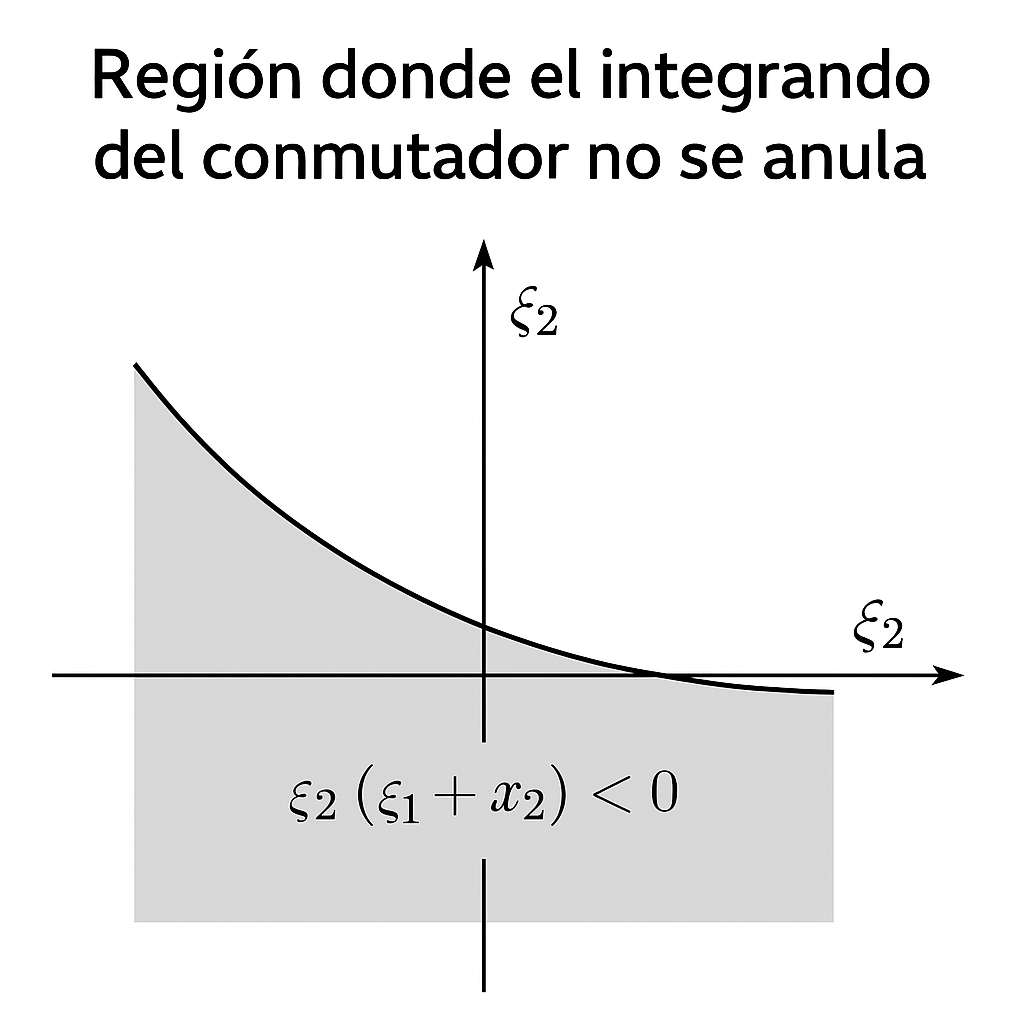
\includegraphics[scale=0.2]{Diagrama de conmutador en 2D.png}
  \end{center}
  
  En ambos casos es equivalente escribir que $|\xi_{2}|<|\xi_{1}|$, lo que nos invita a utilizar la descomposición de paraproducto con el fin de conseguir una estimación, siendo así aplicando la descomposición tipo paraproducto y la propiedad del soporte en frecuencia, podemos escribir
  \begin{align*}
    D_x^\alpha [H_x, g] D_x^\beta f &=H_{x}\left( \sum_{N>0}D^{\alpha}(P_{N}^{x}gP_{\ll N}^{x}D_{x}^{\beta}f) \right)-\sum_{N>0}D^{\alpha}(P_{N}^{x}gP_{\ll N}^{x}H_{x}D_{x}^{\beta}f)\\
    &\phantom{=}+H_{x}\left(\sum_{N>0}D^{\alpha}(P_{N}^{x}g\tilde{P}_{N}^{x}D_{x}^{\beta}f) \right)-\sum_{N>0}D^{\alpha}(P_{N}^{x}g\tilde{P}_{N}^{x}H_{x}D_{x}^{\beta}f),\\
    &= A_1 + A_2 + A_3 + A_4, 
  \end{align*}
  donde
  \begin{align*}
    A_1 &= H_x \left( \sum_{N>0} D_x^\alpha (P_N^x g \cdot P_{\ll N}^x D_x^\beta f) \right), \\
    A_2 &= - \sum_{N>0} D_x^\alpha (P_N^x g \cdot P_{\ll N}^x H_x D_x^\beta f), \\
    A_3 &= H_x \left( \sum_{N>0} D_x^\alpha (P_N^x g \cdot \tilde{P}_N^x D_x^\beta f) \right), \\
    A_4 &= - \sum_{N>0} D_x^\alpha (P_N^x g \cdot \tilde{P}_N^x H_x D_x^\beta f).
  \end{align*}
  Nota: cabe recalcar que $P_{\ll N}^{x}f=\sum_{M\ll N}P_{M}^{x}f$ y $\tilde{P}_{N}^{x}f=\sum_{M\sim N}P_{M}^{x}f$.

\subsection*{Estimación del término $A_1$}
  Recordamos que
  \begin{align*}
    A_1 = H_x\left( \sum_{N > 0} D_x^\alpha \left( P_N^x g \cdot P_{\ll N}^x D_x^\beta f \right) \right),
  \end{align*}
  Como $H_x$ es un operador acotado en $L^p(\mathbb{R})$, basta estimar
  \begin{align*}
    \norm{A_1}_{L^p}
    &\lesssim \left\| \sum_{N > 0} D_x^\alpha \left( P_N^x g \cdot P_{\ll N}^x D_x^\beta f \right) \right\|_{L^p}.
  \end{align*}
  Aplicamos la desigualdad de Littlewood-Paley:
  \begin{align*}
    \norm{\sum_{N} D_x^\alpha \left( P_N^x g \cdot P_{\ll N}^x D_x^\beta f \right)}_{L^p}
    &\lesssim \norm{\left( \sum_{N} |D_x^\alpha (P_N^x g \cdot P_{\ll N}^x D_x^\beta f)|^2 \right)^{1/2}}_{L^p}.
  \end{align*}
  Dado que $P_N^x g$ oscila en frecuencia $\sim N$ y $P_{\ll N}^x D_x^\beta f$ es suave (frecuencias mucho menores que $N$), aplicamos la derivada al factor oscilante:
  \begin{align*}
    |D_x^\alpha (P_N^x g \cdot P_{\ll N}^x D_x^\beta f)(x)|
    &\lesssim |D_x^\alpha P_N^x g(x)| \cdot |P_{\ll N}^x D_x^\beta f(x)|.
  \end{align*}
  Como $P_N^x g$ vive en frecuencia $\sim N$, se cumple que
  \begin{align*}
    |D_x^\alpha P_N^x g(x)| &\lesssim N^\alpha |P_N^x g(x)|.
  \end{align*}
  Por propiedades de Fourier, tenemos $P_N^x g \sim N^{-1} \partial_x P_N^x g$, y por tanto
  \begin{align*}
    |P_N^x g(x)| &\lesssim N^{-1} M(\partial_x g)(x),
  \end{align*}
  usando la acotación de $P_N^x$ por el operador maximal.
  Entonces
  \begin{align*}
    |D_x^\alpha (P_N^x g \cdot P_{\ll N}^x D_x^\beta f)(x)|
    &\lesssim N^\alpha \cdot N^{-1} \cdot M(\partial_x g)(x) \cdot |P_{\ll N}^x D_x^\beta f(x)| \\
    &= N^{-\beta} \cdot M(\partial_x g)(x) \cdot |P_{\ll N}^x D_x^\beta f(x)|.
  \end{align*}
  Aplicamos ahora el operador maximal también a $P_{\ll N}^x D_x^\beta f$:
  \begin{align*}
    |P_{\ll N}^x D_x^\beta f(x)|
    &\leq M(P_{\ll N}^x D_x^\beta f)(x),
  \end{align*}
  y obtenemos:
  \begin{align*}
    |D_x^\alpha (P_N^x g \cdot P_{\ll N}^x D_x^\beta f)(x)|&\lesssim N^{-\beta} M(\partial_x g)(x) \cdot M(P_{\ll N}^x D_x^\beta f)(x).
  \end{align*}
  Sumando en $N$, se concluye:
  \begin{align*}
    \left(\sum_{N>0}|D_x^\alpha (P_N^x g \cdot P_{\ll N}^x D_x^\beta f)(x)|^{2}\right)^{\frac{1}{2}}&\lesssim  M(\partial_x g)(x)\left(\sum_{N}N^{-2\beta}|M(P_{\ll N}^x D_x^\beta f)(x)|^{2}\right)^{\frac{1}{2}}.
  \end{align*}
  Aplicando la desigualdad de Fefferman-Stein:
  \begin{align*}
    \norm{M(\partial_x g)(x)\left(\sum_{N}N^{-2\beta}|M(P_{\ll N}^x D_x^\beta f)(x)|^{2}\right)^{\frac{1}{2}}}_{L^{p}}\leq \norm{M(\partial_x g)(x)\left(\sum_{N}N^{-2\beta}|P_{\ll N}^x D_x^\beta f(x)|^{2}\right)^{\frac{1}{2}}.}_{L^p}
  \end{align*}
  Finalmente, aplicando una reindexación que nos permita deshacernos del $N^{-2\beta}$ usamos la desigualdad de Littlewood-Paley y que el operador maximal es un operador acotado se puede afirmar que
  \begin{align*}
    \|A_1\|_{L^p} \lesssim \norm{\partial_x g}_{L^\infty} \norm{f}_{L^p}.   
  \end{align*}
  Lo que nos permite concluir la estimación del término $A_1$.
  
\subsection*{Estimación del término $A_2$}
  La estimación de $A_2$ sigue exactamente los mismos pasos que la de $A_1$, ya que $H_x$ es un operador lineal acotado en $L^p$, y aparece aplicado sobre $f$ antes del producto. Observamos que:
  \begin{align*}
    A_2 = - \sum_{N > 0} D_x^\alpha (P_N^x g \cdot P_{\ll N}^x H_x D_x^\beta f).
  \end{align*}
  Como $H_x$ conmuta con las proyecciones y es acotado, podemos reemplazar $f$ por $H_x f$ en la estimación anterior. Por tanto:
  \begin{align*}
    \norm{A_2}_{L^p} \lesssim \norm{\partial_x g}_{L^\infty} \norm{H_x f}_{L^p} \lesssim \norm{\partial_x g}_{L^\infty}\norm{f}_{L^p}.   
  \end{align*}
  Lo que nos permite concluir con la estimación del término $A_2$.

\subsection*{Estimación del término $A_3$}
  Recordamos que
  \begin{align*}
    A_3 = H_x\left( \sum_{N > 0} D_x^\alpha \left( P_N^x g \cdot \tilde{P}_N^x D_x^\beta f \right) \right),
  \end{align*}
  donde $\tilde{P}_N^x = \sum_{M : N/8 \leq M \leq 8N} P_M^x$ es una proyección sobre frecuencias comparables a $N$. Como $H_x$ es acotado en $L^p(\mathbb{R})$, basta estimar
  \begin{align*}
    \norm{A_3}_{L^p}&\lesssim \norm{ \sum_{N > 0} D_x^\alpha \left( P_N^x g \tilde{P}_N^x D_x^\beta f \right)}_{L^p}.
  \end{align*}
  Aplicamos la desigualdad de Littlewood-Paley:
  \begin{align*}
    \norm{\sum_{N} D_x^\alpha \left( P_N^x g \cdot \tilde{P}_N^x D_x^\beta f \right)}_{L^p}&\lesssim \norm{\left( \sum_{N} |D_x^\alpha (P_N^x g \cdot \tilde{P}_N^x D_x^\beta f)|^2 \right)^{1/2}}_{L^p}.
  \end{align*}
  Dado que tanto $P_N^x g$ como $\tilde{P}_N^x D_x^\beta f$ oscilan en frecuencias comparables $\sim N$, el producto también vive en frecuencia $\sim N$, y por tanto,
  \begin{align*}
    |D_x^\alpha (P_N^x g \cdot \tilde{P}_N^x D_x^\beta f)(x)|&\lesssim N^\alpha |P_N^x g(x)| \cdot |\tilde{P}_N^x D_x^\beta f(x)|.
  \end{align*}
  Aplicamos ahora el operador maximal a ambos factores:
  \begin{align*}
    |P_N^x g(x)| &\leq M(P_N^x g)(x), \\
    |\tilde{P}_N^x D_x^\beta f(x)| &\leq M(\tilde{P}_N^x D_x^\beta f)(x).
  \end{align*}
  Así, concluimos que
  \begin{align*}
    |D_x^\alpha (P_N^x g \cdot \tilde{P}_N^x D_x^\beta f)(x)|
    &\lesssim N^\alpha M(P_N^x g)(x) \cdot M(\tilde{P}_N^x D_x^\beta f)(x).
  \end{align*}
  Sumando en $N$, se obtiene
  \begin{align*}
    \left(\sum_{N > 0} |D_x^\alpha (P_N^x g \cdot \tilde{P}_N^x D_x^\beta f)(x)|^2\right)^{1/2}&\lesssim \left( \sum_{N} N^{2\alpha} |M(P_N^x g)(x)|^2 \cdot |M(\tilde{P}_N^x D_x^\beta f)(x)|^2 \right)^{1/2}.
  \end{align*}
  Aplicamos la desigualdad de Cauchy-Schwarz en la suma
  \begin{align*}
    &\left( \sum_{N} N^{2\alpha} |M(P_N^x g)(x)|^2 \cdot |M(\tilde{P}_N^x D_x^\beta f)(x)|^2 \right)^{1/2} \\
    &\leq \left( \sum_N N^{2\alpha} |M(P_N^x g)(x)|^2 \right)^{1/2} \cdot \left( \sum_N |M(\tilde{P}_N^x D_x^\beta f)(x)|^2 \right)^{1/2}.
  \end{align*}
  Aplicando la desigualdad de Fefferman-Stein y que el operador maximal es acotado en $L^{\infty}$ en cada término, y luego Littlewood-Paley
  \begin{align*}
    \norm{\left( \sum_N N^{2\alpha} |M(P_N^x g)|^2 \right)^{1/2}}_{L^\infty} &\lesssim \norm{\left( \sum_N N^{2\alpha} |P_N^x g|^2 \right)^{1/2}}_{L^\infty}, \\
    \norm{\left( \sum_N |M(\tilde{P}_N^x D_x^\beta f)|^2 \right)^{1/2}}_{L^p} &\lesssim \norm{\left( \sum_N |\tilde{P}_N^x D_x^\beta f|^2 \right)^{1/2}}_{L^p}.
  \end{align*}
  En conjunto, estimando como lo hicimos anteriormente la $P_{N}^{x}g\sim \frac{1}{N}\partial_{x}g$ se concluye que
  \begin{align*}
    \norm{A_3}_{L^p} \lesssim \norm{\partial_{x}g}_{\infty}\norm{f}_{L^p},
  \end{align*}
  lo cual nos permite concluir la estimación del término $A_3$.

\subsection*{Estimación del término $A_4$}
  La estimación de $A_4$ sigue el mismo esquema que la del término $A_3$, ya que involucra la interacción de frecuencias comparables, pero ahora el operador $H_x$ aparece aplicado a $f$ antes del producto. Observamos que:
  \begin{align*}
    A_4 = - \sum_{N > 0} D_x^\alpha (P_N^x g \cdot \tilde{P}_N^x H_x D_x^\beta f).
  \end{align*}
  Como $H_x$ conmuta con las proyecciones y es acotado en $L^p$, podemos reemplazar $f$ por $H_x f$ en la estimación del término $A_3$. Por tanto:
  \begin{align*}
    \norm{A_4}_{L^p} \lesssim \norm{ \partial_x g}_{L^\infty} \cdot \norm{ H_x f}_{L^p} \lesssim \norm{\partial_x g}_{L^\infty} \cdot \norm{f}_{L^p}.
  \end{align*}
  Lo que nos permite concluir con la estimación del término $A_4$ y por ende el resultado propuesto. 
%%%%%%%%%%%%%%%%%%%%%%%%%%%%%%%%%%%%%%%%%%%%%%%%%%
\section{Implicaciones}
  El resultado obtenido establece la estimación
  \begin{align*}
    \| [H_x D_x^\alpha, g] D_x^\beta f \|_{L^p} \lesssim \| \partial_x g \|_{L^\infty} \cdot \|f\|_{L^p},
  \end{align*}
  donde $\alpha + \beta = 1$. Esta desigualdad tiene varias consecuencias importantes tanto desde el punto de vista teórico como aplicado. A continuación se resumen algunas implicaciones relevantes 
  \begin{enumerate}
    \item La desigualdad muestra que la irregularidad del conmutador está completamente controlada por la derivada de $g$. Aunque el operador $H_x D_x^\alpha$ es no local, el efecto de conmutar con una función queda dominado por $\|\partial_x g\|_{L^\infty}$.
    \item Este tipo de estimaciones aparece naturalmente en el análisis de ecuaciones no lineales dispersivas, como las ecuaciones de Benjamin–Ono, KdV o KP, donde se presentan operadores singulares actuando sobre productos de funciones. El control del conmutador es crucial para garantizar que no haya pérdida de derivadas al cerrar estimaciones de energía.
    \item La estructura del conmutador tiene relación con los operadores pseudo-diferenciales. En particular, si $T_m$ es el operador de Fourier con símbolo $m(\xi) = |\xi|^\alpha \operatorname{sign}(\xi)$, se tiene que
      \begin{align*}
        [T_m, g] f \approx T_{m \cdot \partial_x g} f,
      \end{align*}
      por lo que este resultado puede verse como un modelo concreto de ese comportamiento.
    \item La estimación también puede interpretarse como una versión particular del teorema de Coifman–Meyer para conmutadores, pero bajo hipótesis más suaves. En lugar de asumir que $g \in \mathrm{BMO}$, aquí basta con que $\partial_x g \in L^\infty$, lo cual es más accesible y útil en aplicaciones concretas.
  \end{enumerate}
%%%%%%%%%%%%%%%%%%%%%%%%%%%%%%%%%%%%%%%%%%%%%%%
\section{Conclusiones}
En este trabajo se ha demostrado, con todo detalle, la estimación
\begin{align*}
  \| [H_x D_x^\alpha, g] D_x^\beta f \|_{L^p} \lesssim \| \partial_x g \|_{L^\infty} \cdot \|f\|_{L^p},
\end{align*}
donde $\alpha + \beta = 1$ y $1 < p < \infty$. La demostración se apoyó en herramientas fundamentales del análisis armónico, como la descomposición de Littlewood–Paley, la teoría de operadores singulares, el operador maximal de Hardy–Littlewood, el teorema de Fefferman–Stein y técnicas de conmutadores.

Cada uno de los términos en los que se descompone el conmutador fue tratado cuidadosamente, analizando los distintos regímenes de interacción entre las frecuencias de $g$ y $f$ (baja-alta, alta-baja y comparable). Se verificó que en todos los casos, el efecto del conmutador se puede controlar únicamente por la derivada de $g$ y la norma $L^p$ de $f$.

Este resultado es representativo de una clase de estimaciones que juegan un papel central en el estudio de ecuaciones no lineales dispersivas, donde la interacción entre operadores singulares y productos de funciones requiere un tratamiento delicado. Además, sirve como modelo para entender conmutadores de operadores pseudo-diferenciales con multiplicadores suaves, y como una versión particular accesible de la teoría general de Coifman–Meyer.

En conjunto, la estimación obtenida permite asegurar que la operación de conmutar un operador singular con una función multiplicadora no introduce irregularidades inesperadas, siempre que $g$ tenga derivada acotada. Esto la convierte en una herramienta eficaz para el análisis de problemas no lineales donde intervienen estructuras similares.
%%%%%%%%%%%%%%%%%%%%%%%%%%%%%%%%%%%%%%%%%%%%%%%
\newpage
\nocite{*}
\printbibliography

\end{document}
